\section{Results}\label{sec:results}
% Testen van het weerstation (ventilator, zon, etc.)
% Victron verifiëren via CCGX, vermogens van de twee multiplus systemen
% GPIO's
% Robuustheidstest (random dingen uitpluggen, langer laten draaien, etc.)
% valgrind
% manual in appendix noemen

\subsection{Weather station}
To verify correct functionality of both the weather station and the communication with the ODROID, a simple test setup was conducted to test all the used sensors. Most sensors could be read at any time (temperature, humidity, air pressure). However, both the radiation sensor and wind sensors would register zero because there was not enough light and wind to trigger these sensors. The weather station was set up at the window on a bright day to test the radiation sensor, and a fan was placed to check if the wind was received correctly. During these tests, all sensor values were correctly read and sent to the server. This confirmed the functionality of both the weather station and the communication with the server.

\subsection{Victron system}\label{sec:victron_results}
For reading the registers of the Victron system the Modbus libraries are used. By printing the read values to the screen it was easily verified that the ODROID was able to read the Victron system.\\

To determine what the registers with respect to the power represent, a load was connected to the system. An easy way to do this is by connecting a large power resistor to the system. The power dissipated in this resistor was recognized as DC power on the Victron system. \\

%However, it was not possible to read this register using the  ODROID.\\
Some 230V sockets are also connected to the Victron system. The ODROID, router and display are connected to these sockets. By switching the display on, an increase in AC power was detected in one of the MultiPlus slaves (slave ID 0). The other MultiPlus slave, however, did not register it, so it was clear that although they are the same physical device, they do register different information.\\

To find out what they are measuring, the systems were both monitored for roughly a day. The results of input power can be found in \Cref{fig:MultiPlus_inputs}. The peak of roughly 1.8kW is the moment that the Victron system starts charging the batteries with energy from the grid.\\

\begin{figure}
\centering
\begin{subfigure}{.5\textwidth}
  \centering
  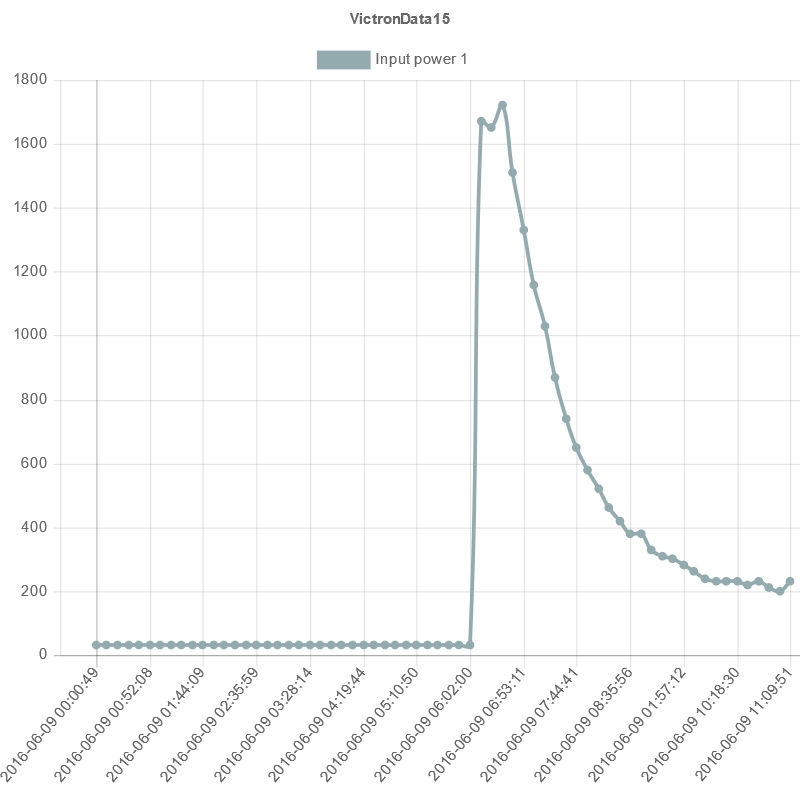
\includegraphics[width=.95\linewidth]{images/Input_power_30W.png}
  \caption{MultiPlus on slave ID 0}
  \label{fig:MultiPlus_input_30W}
\end{subfigure}%
\begin{subfigure}{.5\textwidth}
  \centering
  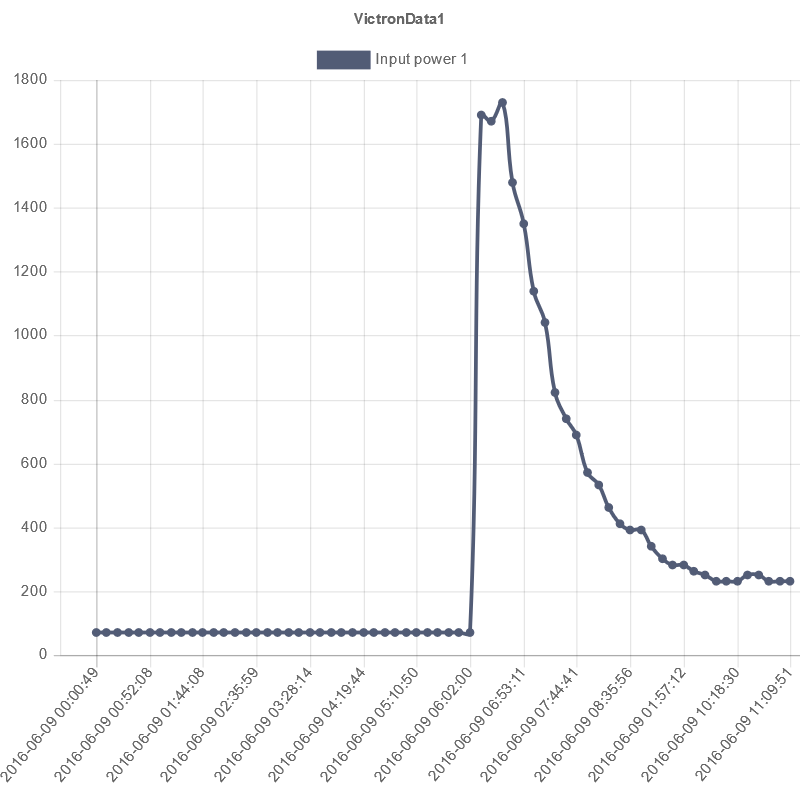
\includegraphics[width=.95\linewidth]{images/Input_power_70W.png}
  \caption{MultiPlus on slave ID 246}
  \label{fig:MultiPlus_input_70W}
\end{subfigure}
\caption{Input power of the MultiPlus slaves}
\label{fig:MultiPlus_inputs}
\end{figure}

At first, these graphs look identical. However, closer inspection reveals that the device at slave ID 0 has a standby power of 30W, and the other device has a standby power of 70W. There are also minor differences in the peak during charging. Similar results are found for the output powers.\\

Concluding, it is thought that MultiPlus devices both monitor the AC power regarding the batteries. External AC connections (e.g. router, local screen, etc.) are found in the MultiPlus device with slave ID 0, and all internal AC power (all the Victron devices) are monitored by the MultiPlus device with slave ID 246. The last guess is mainly based on the fact that the 70W standby does not change when anything is connected, and 70W is in the order of power usage of the Victron systems.\\

Another important result is that it is not possible to read all the registers that are mentioned in the register list. Most of these unreadable registers are a result of devices that are not connected due to the modularity of the Victron system. Moreover, it was not possible to read the state of health of the batteries on register address 304, despite the fact that there is a battery management system inside. It is unclear why this register cannot be read, but it is likely that it is simply not supported by the batteries that are used.

\subsection{Chargers}
The chargers are tested in a conceptual way by controlling the LEDs connected to the GPIO pins. Beforehand it is of course necessary to test the driver that is used for the LED as shown in \Cref{fig:leddriver}. During the test a 5V and 3.3V supply were used to deliver the energy.\\

First, the value of the highest possible Rb was determined. When using a 22k$\Omega$ resistance the transistor did not function as desired, hence a smaller resistor needed to be selected. A 10k$\Omega$ resistance Rb was enough to ensure that sufficient current could enter the base of the transistor. However, the current through the base is inversely proportional to the resistance Rb. This is a result of the constant voltage drop of about 0.7V over the base-emitter junction. A smaller Rb thus results in a higher base current and hence an increased current drawn from the GPIO pin.\\

When the transistor is in saturation, a voltage of about 0.69V was measured at the base terminal. The voltage at the collector terminal was about 0.073V. Now it can be concluded that the transistor is indeed in saturation. At the base, the voltage is higher than at the collector and the emitter. Using the fact that the P2N2222A is an NPN transistor it means that both the base-emitter junction and the base-collector junction are forward biased. Using these measurements and the value of Rb the base current is $\frac{3.3-0.69}{10k}=0.26mA=260\mu A$.\\

A voltage of 1.69V was measured over Rc; hence the current through the LED equals 5.1mA which is enough to make the LED clearly visible. By using the state of the chargers fetched from the server, the GPIO pins were set to a logic 0 or 1. A change in the state of a charger in the database was indicated on the LEDs in less than 1.5 seconds.\\

The FSM controlling the chargers was tested by connecting both the LED array (described above) and the switch described in \Cref{fig:cable_detect}. All the state changes were tested on their functionality (by printing all current states) as well as their timing (counting the number of cycles until a state change). This resulted in no significant problems, however it was evident that not all functionality was present. The main issue was that the charger would not respond to the administrator turning off a charger. This was solved by making an \verb|if|-statement that sets the local charger state to OFF for all chargers that are set to 0 on the server. This force-statement resets all timers used in any of the states.

\subsection{Solar panel temperature sensors}
The temperature probes were easily tested by reading the registers from the ADAM module to which they are connected. Using the Modbus routines to read registers data was obtained. During the test, only one temperature sensor was connected (there are 5 more slots available to connect temperature sensors). From the registers that were not connected to a temperature sensor, the value $2^{16}-1=65535$ was returned, which means it is unconnected but functioning. Register 4, to which a sensor was connected, returned a value between $0$ and $2^{16}-1$. Using the mapping as described in \Cref{sec:temp_sensors} this value was mapped to a temperature, which indeed corresponded to the current room temperature.

\subsection{Local Display}
The file that contains the data for the local display is correctly generated every 15 seconds by the display function. The webpage that is going to be displayed in the actual charging station is yet to be finished by another team in project SUNRISE, thus the actual implementation of reading this file is yet to be finalized. However, all other necessary precautions have been taken regarding this webpage: the ability to run WebGL and the ability to automatically boot all display programs (see \Cref{sec:bash_results}). A small script was also written to test the reading of the file, and the data was displayed and refreshed without any issues (see \Cref{fig:test_display}).

\begin{figure}[!ht]
  \centering
    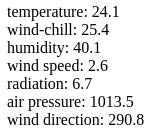
\includegraphics[width=0.15\textwidth]{images/test_display.png}
      \caption{Output of the test webpage}\label{fig:test_display}
\end{figure}

\subsection{Bash}\label{sec:bash_results}
The bash scripts all function as designed. The scripts can boot the browser on startup, boot and reboot the C-code, ensure there are not too many remote desktops connected and hide the mouse so it does not display on the local display.

\subsection{General testing}
\subsubsection{Memory leaks}
Although the C-code was written with the utmost care, chances are that not all memory allocations are freed. Because the code is running 24/7, any memory leaks would sooner or later become an issue for the system. It was therefore necessary to ensure no memory leaks were created by the code.\\

A Linux tool called ``Valgrind'' \cite{valgrind} was used to check the code of any memory leaks. Valgrind has a tool specifically designed for this: memcheck. Two memory leaks were found by this tool, both caused during casting of data. The problem was that a variable that would contain the result of the casts function had memory allocated. However, the same memory allocation was done within the cast function. The earlier mentioned variable would be overwritten by the data of the cast function, causing it to lose the location of the memory that was allocated to it. A memory leak was mentioned by Valgrind, and some manual searching of the code led to the core of the problem.\\

In later stages of the design, it was decided that memory allocations should be removed alltogether (if possible). This is further explained in \Cref{sec:malloc}.

\subsubsection{Long term tests}
The ability of the code to run for a longer time is a very important aspect to test. Multiple tests were conducted in which the code would run overnight by using Valgrind. During these test all available functionality of the code was used (reading the devices, controlling the GPIO pins and sending and receiving data from the server). Both tests resulted in a failure of the code. The database showed that data had been received up until 3 a.m. and then nothing more was received. The terminal window in which the program was running showed that wrong data was received on the ODROID about the state of the chargers. Only zeroes and ones should be received, however some random values were received which caused the program to crash. This is probably a result of a kind of reset that is done every night on the server of TU Delft. The server code did return a null pointer when no data was received, but this result was not checked and was therefore still written to the pins. This was probably random memory data, which finally crashed the program.\\

In the end, roughly 6 long-term tests were conducted, ranging between 24 and 96 hours. The duration of a full cycle (\Cref{fig:code_overview}) was not very constant, but it did not deviate more than about 15 seconds from the 5 or 10 minute cycle. This will not be a major issue since this deviation did not accumulate after several cycles.\\

\subsubsection{Robustness tests}\label{sec:robustness_tests}
To guarantee robustness, it was important to unplug and replug all ODROID connections multiple times. This reveiled some minor bugs regarding server connectivity, but ultimately resulted in sturdy code that will simply reconnect whenever a device becomes available again.\\

A more interesting result occurred when unplugging both Modbus RTU connections (temperature probes and weather station). This sometimes resulted in the devices not being found after reconnecting. It was soon noticed that the order in which the devices are connected is important. Due to limited development time, it was not considered important enough to dynamically allocate these USB connections to make the ODROID independent of connection order (if at all possible). Until that time, the USB of the temperature sensors should be plugged in before the weather station.